\documentclass[12pt,letterpaper]{article}
\usepackage[utf8]{inputenc}
\usepackage{amsmath}
\usepackage{amsfonts}
\usepackage{amssymb}
\usepackage{float}
\usepackage[margin=0.75in]{geometry}
\usepackage[parfill]{parskip}
\usepackage{graphicx}
\graphicspath{ {images/} }

\usepackage{fancyhdr}
 
\pagestyle{fancy}
\fancyhf{}
\lhead{Andrew Wintenberg}
\rhead{{Page \thepage}}

\linespread{1}

\author{Andrew Wintenberg}
\title{Goldwater Research}
\begin{document}

\begin{center}
{\Large \textbf{Homework 1 : ECE 472 }}

{\large Andrew Wintenberg}

{\today}
\end{center}

\thispagestyle{empty}

\section{Introduction}

The objective of this homework was to implement pixel level image operations and analyze their effects on image features. Specifically, the operations performed were scaling, inversion, logarithm, exponential, power law, and histogram equalization. Using the provided image of a woman's face (pictured below), the appearance of the resulting images and their histograms were compared to describe the effect of the operations.

All computations were performed using a personal C library written for this course. Histogram plots were generated using Matlab with data exported from the library. All images were represented with 8-bit grayscale pixels and stored in the BMP file format. For each operation, the resulting image and histogram are pictured in the relevant section.


\begin{figure}[ht]
\centering
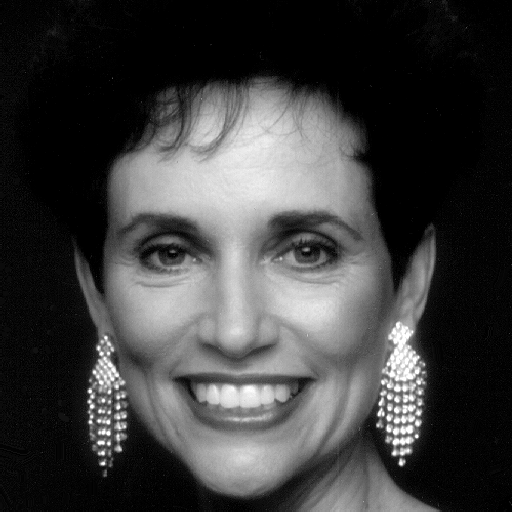
\includegraphics[scale=1.75]{woman/woman} \hspace{0.5cm} \includegraphics[scale=0.6]{woman/histogram_images/base_hist}
\caption{\small{The original image and its histogram on which operations were performed}
\label{fig:base} }
\end{figure}

\newpage

\section{Results}

\subsection{Divide Intensity by 2}
For each pixel in the image, the intensity of the pixel was divided 2. As expected, the image becomes significantly dimmer and the histogram is twice as narrow and twice as tall.

\begin{figure}[ht]
\centering
\includegraphics[scale=0.135]{woman/scale} \hspace{0.5cm} \includegraphics[scale=0.6]{woman/histogram_images/scale_hist}
\caption{\small{The image and its histogram after scaling}
\label{fig:div2} }
\end{figure}

\vspace{-0.5cm}

\subsection{Scaling}
The range of the image is mapped linearly to the entire range of intensities $[0, 255]$. The image the operation was performed on was the image with intensities divided by two as to provide appreciable results. We can see that the dim image was mapped to an image that occupies the entire range of intensities, but the histogram is now sparser.
\begin{figure}[ht]
\centering
\includegraphics[scale=0.135]{woman/scale_range} \hspace{0.5cm} \includegraphics[scale=0.6]{woman/histogram_images/scale_range_hist}
\caption{\small{The image and its histogram after dividing intensity by 2}
\label{fig:scale} }
\end{figure}



\subsection{Inversion}
For each pixel in the image, the intensity of the pixel was inverted or equivalently subtracted from the maximum intensity 255. The dark portions of the image are now light and vice versa. New detail is visible such as the varying intensities on the teeth. The histogram is mirrored.

\begin{figure}[ht]
\centering
\includegraphics[scale=0.135]{woman/inv} \hspace{0.5cm} \includegraphics[scale=0.6]{woman/histogram_images/inv_hist}
\caption{\small{The image and its histogram after inversion}
\label{fig:inv} }
\end{figure}

\vspace{-0.5cm}

\subsection{Logarithm}
Pixels are mapped according to $s = c \log(1 + r)$ where $c$ is chosen to preserve the range of intensities. There is more detail in the dim areas of the image, exposing noise in the background. Also the light areas are compressed with less detail. This is reflected in the histogram as well with stretching of the lower part of the histogram.
\begin{figure}[ht]
\centering
\includegraphics[scale=0.135]{woman/log} \hspace{0.5cm} \includegraphics[scale=0.6]{woman/histogram_images/log_hist}
\caption{\small{The image and its histogram after performing the logarithm}
\label{fig:log} }
\end{figure}



\subsection{Exponentiation}
Pixels are mapped according to $s = b^r - 1$ where $b$ is chosen to preserve the range of intensities. There is more detail in the bright areas of the image and less in the dark. This is reflected in the histogram with stretching of the higher part of the histogram.
\begin{figure}[ht]
\centering
\includegraphics[scale=0.135]{woman/exp} \hspace{0.5cm} \includegraphics[scale=0.6]{woman/histogram_images/exp_hist}
\caption{\small{The image and its histogram after exponentiation}
\label{fig:exp} }
\end{figure}

\vspace{-0.5cm}

\subsection{Logarithm and Exponentiation Histogram Equalization}
The images produced from the logarithm and exponentiation operations were histogram equalized to approximately achieve a uniform histogram. This was done by computing the cumulative distribution of the normalized histograms and then using this function as a pixel operation. Pixels were then scaled by a constant 255 to map the probabilities to intensities. No image scaling was performed after this. This operation spreads the intensities of the image out, resulting in images that resemble the original after being distorted by the logarithm and exponential.

\begin{figure}[ht]
\centering
\includegraphics[scale=0.135]{woman/logEqualized} \hspace{0.5cm} \includegraphics[scale=0.6]{woman/histogram_images/log_equ_hist}
\caption{\small{The logarithm image and its histogram after performing histogram equalization}
\label{fig:log_equ} }
\end{figure}

\begin{figure}[ht]
\centering
\includegraphics[scale=0.135]{woman/expEqualized} \hspace{0.5cm} \includegraphics[scale=0.6]{woman/histogram_images/exp_equ_hist}
\caption{\small{The exponential image and its histogram after performing histogram equalization}
\label{fig:exp_equ} }
\end{figure}

\vspace{-0.5cm}

\subsection{Power Law (Gamma)}
For various values of gamma $\Gamma$, pixels are mapped according to $s = c r^{\Gamma}$ where $c$ is chosen to preserve the range of the intensities. For $\Gamma < 1$ the images approximate the logarithm map while for $\Gamma > 1$ the images approximate the exponential map. Of course for $\Gamma = 1$ this operation is the identity, not changing the base image. The values of $\Gamma$ pictured below are $0.125, 0.25, 0.5, 1, 2, 4, 8$. For lower values of $\Gamma$, the image is generally brighter and the the noise in the dark background is emphasized. For larger values of $\Gamma$, the image is darker and there is more contrast in the brighter areas.

\begin{figure}[ht]
\centering
\includegraphics[scale=0.135]{{woman/gamma/gamma0.13}.png} \hspace{0.5cm} \includegraphics[scale=0.6]{{woman/histogram_images/gamma/gamma0.13_hist}.png}
\caption{\small{The image and its histogram after performing the power law with $\Gamma = 0.125$}
\label{fig:gamma013} }
\end{figure}

\begin{figure}[ht]
\centering
\includegraphics[scale=0.135]{{woman/gamma/gamma0.25}.png} \hspace{0.5cm} \includegraphics[scale=0.6]{{woman/histogram_images/gamma/gamma0.25_hist}.png}
\caption{\small{The image and its histogram after performing the power law with $\Gamma = 0.25$}
\label{fig:gamma025} }
\end{figure}

\begin{figure}[ht]
\centering
\includegraphics[scale=0.135]{{woman/gamma/gamma0.50}.png} \hspace{0.5cm} \includegraphics[scale=0.6]{{woman/histogram_images/gamma/gamma0.50_hist}.png}
\caption{\small{The image and its histogram after performing the power law with $\Gamma = 0.5$}
\label{fig:gamma050} }
\end{figure}

\begin{figure}[ht]
\centering
\includegraphics[scale=0.135]{{woman/gamma/gamma1.00}.png} \hspace{0.5cm} \includegraphics[scale=0.6]{{woman/histogram_images/gamma/gamma1.00_hist}.png}
\caption{\small{The image and its histogram after performing the power law with $\Gamma = 1$}
\label{fig:gamma100} }
\end{figure}


\begin{figure}[ht]
\centering
\includegraphics[scale=0.135]{{woman/gamma/gamma2.00}.png} \hspace{0.5cm} \includegraphics[scale=0.6]{{woman/histogram_images/gamma/gamma2.00_hist}.png}
\caption{\small{The image and its histogram after performing the power law with $\Gamma = 2$}
\label{fig:gamma200} }
\end{figure}

\begin{figure}[ht]
\centering
\includegraphics[scale=0.135]{{woman/gamma/gamma4.00}.png} \hspace{0.5cm} \includegraphics[scale=0.6]{{woman/histogram_images/gamma/gamma4.00_hist}.png}
\caption{\small{The image and its histogram after performing the power law with $\Gamma = 4$}
\label{fig:gamma400} }
\end{figure}

\begin{figure}[ht]
\centering
\includegraphics[scale=0.135]{{woman/gamma/gamma8.00}.png} \hspace{0.5cm} \includegraphics[scale=0.6]{{woman/histogram_images/gamma/gamma8.00_hist}.png}
\caption{\small{The image and its histogram after performing the power law with $\Gamma = 8$}
\label{fig:gamma800} }
\end{figure}


\clearpage


\subsection{Power Law (Gamma) Histogram Equalization}
The images output from the power law operation were then histogram equalized as with the logarithm and exponential. The results are similar with the equalized images more smoothly occupying the range of intensities and resembling the original image.

\begin{figure}[H]
\centering
\includegraphics[scale=0.135]{{woman/gamma/gamma0.13_Equalized}.png} \hspace{0.5cm} \includegraphics[scale=0.6]{{woman/histogram_images/gamma/gamma0.13_equ_hist}.png}
\caption{\small{The equalized image and its histogram after performing the power law with $\Gamma = 0.125$}
\label{fig:gamma013_equ} }
\end{figure}

\begin{figure}[ht]
\centering
\includegraphics[scale=0.135]{{woman/gamma/gamma0.25_Equalized}.png} \hspace{0.5cm} \includegraphics[scale=0.6]{{woman/histogram_images/gamma/gamma0.25_equ_hist}.png}
\caption{\small{The equalized image and its histogram after performing the power law with $\Gamma = 0.25$}
\label{fig:gamma025_equ} }
\end{figure}

\begin{figure}[ht]
\centering
\includegraphics[scale=0.135]{{woman/gamma/gamma0.50_Equalized}.png} \hspace{0.5cm} \includegraphics[scale=0.6]{{woman/histogram_images/gamma/gamma0.50_equ_hist}.png}
\caption{\small{The equalized image and its histogram after performing the power law with $\Gamma = 0.5$}
\label{fig:gamma050_equ} }
\end{figure}

\begin{figure}[ht]
\centering
\includegraphics[scale=0.135]{{woman/gamma/gamma1.00_Equalized}.png} \hspace{0.5cm} \includegraphics[scale=0.6]{{woman/histogram_images/gamma/gamma1.00_equ_hist}.png}
\caption{\small{The equalized image and its histogram after performing the power law with $\Gamma = 1$}
\label{fig:gamma100_equ} }
\end{figure}


\begin{figure}[ht]
\centering
\includegraphics[scale=0.135]{{woman/gamma/gamma2.00_Equalized}.png} \hspace{0.5cm} \includegraphics[scale=0.6]{{woman/histogram_images/gamma/gamma2.00_equ_hist}.png}
\caption{\small{The equalized image and its histogram after performing the power law with $\Gamma = 2$}
\label{fig:gamma200_equ} }
\end{figure}

\begin{figure}[ht]
\centering
\includegraphics[scale=0.135]{{woman/gamma/gamma4.00_Equalized}.png} \hspace{0.5cm} \includegraphics[scale=0.6]{{woman/histogram_images/gamma/gamma4.00_equ_hist}.png}
\caption{\small{The equalized image and its histogram after performing the power law with $\Gamma = 4$}
\label{fig:gamma400_equ} }
\end{figure}

\begin{figure}[ht]
\centering
\includegraphics[scale=0.135]{{woman/gamma/gamma8.00_Equalized}.png} \hspace{0.5cm} \includegraphics[scale=0.6]{{woman/histogram_images/gamma/gamma8.00_equ_hist}.png}
\caption{\small{The equalized image and its histogram after performing the power law with $\Gamma = 8$}
\label{fig:gamma800_equ} }
\end{figure}

\clearpage
 
\section{Conclusion}
In conclusion, the various pixel operations performed on an image can emphasize certain image features and can be described by their transformation of image histograms.

\end{document}